%%
%% This is file `sample-sigconf.tex',
%% generated with the docstrip utility.
%%
%% The original source files were:
%%
%% samples.dtx  (with options: `all,proceedings,bibtex,sigconf')
%% 
%% IMPORTANT NOTICE:
%% 
%% For the copyright see the source file.
%% 
%% Any modified versions of this file must be renamed
%% with new filenames distinct from sample-sigconf.tex.
%% 
%% For distribution of the original source see the terms
%% for copying and modification in the file samples.dtx.
%% 
%% This generated file may be distributed as long as the
%% original source files, as listed above, are part of the
%% same distribution. (The sources need not necessarily be
%% in the same archive or directory.)
%%
%%
%% Commands for TeXCount
%TC:macro \cite [option:text,text]
%TC:macro \citep [option:text,text]
%TC:macro \citet [option:text,text]
%TC:envir table 0 1
%TC:envir table* 0 1
%TC:envir tabular [ignore] word
%TC:envir displaymath 0 word
%TC:envir math 0 word
%TC:envir comment 0 0
%%
%%
%% The first command in your LaTeX source must be the \documentclass
%% command.
%%
%% For submission and review of your manuscript please change the
%% command to \documentclass[manuscript, screen, review]{acmart}.
%%
%% When submitting camera ready or to TAPS, please change the command
%% to \documentclass[sigconf]{acmart} or whichever template is required
%% for your publication.
%%
%%
\documentclass[sigconf,review,anonymous]{acmart}

%%
%% \BibTeX command to typeset BibTeX logo in the docs
\AtBeginDocument{%
  \providecommand\BibTeX{{%
    Bib\TeX}}}

%% Rights management information.  This information is sent to you
%% when you complete the rights form.  These commands have SAMPLE
%% values in them; it is your responsibility as an author to replace
%% the commands and values with those provided to you when you
%% complete the rights form.
\setcopyright{acmlicensed}
\copyrightyear{2024}
\acmYear{2024}
\acmDOI{XXXXXXX.XXXXXXX}

%% These commands are for a PROCEEDINGS abstract or paper.
\acmConference[ICSE '25]{Internation Conference on Software Engineering}{April 27--May 3,
  2025}{Ottawa, Ontario, Canada}
%%
%%  Uncomment \acmBooktitle if the title of the proceedings is different
%%  from ``Proceedings of ...''!
%%
%%\acmBooktitle{Woodstock '18: ACM Symposium on Neural Gaze Detection,
%%  June 03--05, 2018, Woodstock, NY}
\acmISBN{978-1-4503-XXXX-X/18/06}


%%
%% Submission ID.
%% Use this when submitting an article to a sponsored event. You'll
%% receive a unique submission ID from the organizers
%% of the event, and this ID should be used as the parameter to this command.
%%\acmSubmissionID{123-A56-BU3}

%%
%% For managing citations, it is recommended to use bibliography
%% files in BibTeX format.
%%
%% You can then either use BibTeX with the ACM-Reference-Format style,
%% or BibLaTeX with the acmnumeric or acmauthoryear sytles, that include
%% support for advanced citation of software artefact from the
%% biblatex-software package, also separately available on CTAN.
%%
%% Look at the sample-*-biblatex.tex files for templates showcasing
%% the biblatex styles.
%%

%%
%% The majority of ACM publications use numbered citations and
%% references.  The command \citestyle{authoryear} switches to the
%% "author year" style.
%%
%% If you are preparing content for an event
%% sponsored by ACM SIGGRAPH, you must use the "author year" style of
%% citations and references.
%% Uncommenting
%% the next command will enable that style.
%%\citestyle{acmauthoryear}
%%

\usepackage{forest}
\usepackage{amsmath}
\usepackage{xcolor}
\usepackage{hyperref}
\usepackage{tikz}
\usetikzlibrary{quantikz2}
\usepackage{subfigure}
%% end of the preamble, start of the body of the document source.
\begin{document}




%%
%% The "title" command has an optional parameter,
%% allowing the author to define a "short title" to be used in page headers.
\title{Enhancing and Optimizing Grover's Algorithm for Unified Random Sampling of Software Product Lines}

%%
%% The abstract is a short summary of the work to be presented in the
%% article.
\begin{abstract}
This paper improves upon the previous implementations of Grover's algorithm for uniform random sampling in the context of software product lines.
By addressing inefficiencies in quantum circuit design for software product lines (SPLs) we manage to reduce the quantum circuit depth and width significantly.
Additionally we propose novel approaches to designing a Grover oracle for software product lines.
Specifically, we focus on two main tasks: Removing redundant quantum operations that increase computational overhead and introducing lookup tables to optimize qubit usage. 
These improvements were evaluated using SPL models by the BURST benchmarking suite and SPL tool FeatureIDE, measuring both the circuit depth and width.
The results demonstrate that our optimizations lead to substantial reductions in circuit size, particularly for larger feature models, making Grover's algorithm more scalable and efficient for practical applications in SPL testing and management.
\end{abstract}

%%
%% Keywords. The author(s) should pick words that accurately describe
%% the work being presented. Separate the keywords with commas. 
\keywords{Quantum Computing, Grover's Algorithm, Software Product Lines}
%% A "teaser" image appears between the author and affiliation
%% information and the body of the document, and typically spans the
%% page.

\received{11 November 2024}
\received[revised]{dd-mm-yyyy}
\received[accepted]{dd-mm-yyyy}

%%
%% This command processes the author and affiliation and title
%% information and builds the first part of the formatted document.
\maketitle

\section{Introduction}
Software product lines (SPLs) represent an approach to software engineering, facilitating the systematic and efficient management of variations within a family of related software systems. 
SPLs permit the development of a set of features, from which a multitude of product variants can be constructed, thereby addressing the requirements of customers or market segments.
However, this flexibility introduces significant complexity, particularly with regard to testing and verifying the correctness of individual product configurations.

In the context of software product lines, the term \textit{sampling} is used to describe a process through which a subset of the total population of items is selected for further analysis.
Uniform random sampling is of particular importance for unbiased testing, analysis, and quality assurance \cite{plazar-spl-sampling, dutra-sat-sampling, oh-spl-random-sampling, oh-t-wise}, as it ensures that each product variant has an equal chance of being selected, thereby avoiding biases that might lead to incorrect conclusions about the overall product line.

The potential of quantum computing to solve complex problems more efficiently than classical approaches offers promising solutions for many computational challenges, including those found in SPLs.
In this context, Grover's Quantum Algorithm represents a powerful tool for searching unsorted databases or solving satisfiability problems \cite{math11081888, Hangleiter_2023}.
When applied to a Boolean formula representing constraints in an SPL, Grover's algorithm can be employed to identify satisfying configurations with a quadratic speedup compared to brute forcing.
This ability makes it a strong candidate for enabling uniform random sampling in SPLs, as it can efficiently identify valid product configurations from a large space.

Although there already are existing approaches for a quantum implementation, they frequently allow for optimization.
Previous research on the application of Grover's algorithm to SPLs did not fully optimize the quantum circuit, resulting in inefficiencies in gate operations and qubit utilization.
Specifically, the prior implementation failed to remove obsolete gates, such as pairs of X gates that cancel each other out, and did not adequately identify opportunities for qubit reuse, where qubits performing the same function could have been shared rather than redundantly created.
These oversights not only increase the complexity of the quantum circuit but also reduce the overall efficiency and practicality of the quantum algorithm.

This paper builds on the foundational work of previous research \cite{ammermann2023quantumcomputingimproveuniform} by introducing significant improvements to the quantum circuit design for uniform random sampling in SPLs.
By optimizing the quantum gate sequence and implementing effective qubit reuse strategies, we aim to reduce the resource requirements and enhance the performance of Grover's algorithm in this context.
Our contributions not only streamline the quantum computation process but also make the application of quantum algorithms to SPLs more feasible and effective, paving the way for more advanced and efficient quantum software engineering practices.

\section{Background}
This chapter provides the requisite background information for understanding the concepts and techniques utilized in our enhanced quantum implementation for uniform random sampling in software product lines (SPLs).
It covers the necessary fundamentals of SPLs, quantum computing principles, and Grover's algorithm. 
This background chapter will only explain the knowledge needed to understand the improvement implemented and proposed by this paper.

\begin{figure*}
    \centering
    \usetikzlibrary{angles}
\usetikzlibrary{positioning}
\definecolor{drawColor}{RGB}{128 128 128}
\newcommand{\circleSize}{0.25em}
\newcommand{\angleSize}{0.8em}

\forestset{
	/tikz/mandatory/.style={
		circle,fill=drawColor,
		draw=drawColor,
		inner sep=\circleSize
	},
	/tikz/optional/.style={
		circle,
		fill=white,
		draw=drawColor,
		inner sep=\circleSize
	},
	featureDiagram/.style={
		for tree={
			minimum height = 0.6cm,
			text depth = 0,
			draw = drawColor,
			edge = {draw=drawColor},
			parent anchor = south,
			child anchor = north,
			l sep = 2em,
			s sep = 1em,
		}
	},
	/tikz/redColor/.style={
		fill = red!60,
		draw = drawColor
	},
	/tikz/orangeColor/.style={
		fill = orange!50,
		draw = drawColor
	},
	/tikz/yellowColor/.style={
		fill = yellow!50,
		draw = drawColor
	},
	/tikz/darkGreenColor/.style={
		fill = black!30!green,
		draw = drawColor
	},
	/tikz/lightGreenColor/.style={
		fill = green!30,
		draw = drawColor
	},
	/tikz/cyanColor/.style={
		fill = cyan!30,
		draw = drawColor
	},
	/tikz/lightGrayColor/.style={
		fill = black!10,
		draw = drawColor
	},
	/tikz/blueColor/.style={
		fill = blue!50,
		draw = drawColor
	},
	/tikz/magentaColor/.style={
		fill = magenta,
		draw = drawColor
	},
	/tikz/pinkColor/.style={
		fill = pink!90,
		draw = drawColor
	},
	/tikz/abstract/.style={
		fill = blue!85!cyan!5,
		draw = drawColor
	},
	/tikz/concrete/.style={
		fill = blue!85!cyan!20,
		draw = drawColor
	},
	mandatory/.style={
		edge label={node [mandatory] {} }
	},
	optional/.style={
		edge label={node [optional] {} }
	},
	or/.style={
		tikz+={
			\path (.parent) coordinate (A) -- (!u.children) coordinate (B) -- (!ul.parent) coordinate (C) pic[fill=drawColor, angle radius=\angleSize]{angle};
		}	
	},
	/tikz/or/.style={
	},
	alternative/.style={
		tikz+={
			\path (.parent) coordinate (A) -- (!u.children) coordinate (B) -- (!ul.parent) coordinate (C) pic[draw=drawColor, angle radius=\angleSize]{angle};
		}	
	},
	/tikz/alternative/.style={
	},
	/tikz/placeholder/.style={
	},
	collapsed/.style={
		rounded corners,
		no edge,
		for tree={
			fill opacity=0,
			draw opacity=0,
			l = 0em,
		}
	},
	/tikz/hiddenNodes/.style={
		midway,
		rounded corners,
		draw=drawColor,
		fill=white,
		minimum size = 1.2em,
		minimum width = 0.8em,
		scale=0.9
	},
}

\begin{forest}
	featureDiagram
	[Sandwich,concrete[Bread,concrete,mandatory[Full Grain ,concrete,alternative][Toast,concrete][Flatbread,concrete]][Cheese,concrete,optional[Gouda,concrete,optional][Cheddar,concrete,optional]][Meat,concrete,optional[Salami ,concrete,optional][Ham,concrete,optional]]]	
	\matrix [anchor=north west] at (current bounding box.north east) {
		\node [placeholder] {}; \\
	};
	\matrix [draw=drawColor,anchor=north west] at (current bounding box.north east) {
		\node [label=center:\underline{Legend:}] {}; \\
		\node [concrete,label=right:Feature] {}; \\
		\node [mandatory,label=right:Mandatory] {}; \\
		\node [optional,label=right:Optional] {}; \\
			\draw[drawColor] (0.1,0) -- +(-0.2, -0.4);
			\draw[drawColor] (0.1,0) -- +(0.2,-0.4);
			\draw[drawColor] (0,-0.2) arc (240:300:0.2);
		\node [alternative,label=right:Alternative Group] {}; \\	};
	\matrix [below=1mm of current bounding box] {
	\node {\( \text{Full Grain } \Rightarrow \text{Gouda} \land \text{Salami } \)}; \\
	\node {\( \text{Toast} \Rightarrow \text{Gouda} \land \text{Salami } \)}; \\
	};
\end{forest}
    \caption{Feature Model describing a Sandwich with additional constraints.}
    \label{fig:bg:spl:sandwich-imply-model}
\end{figure*}

\subsection{Software Product Lines}
A software product line (SPL) represents a strategic approach to software engineering that prioritizes the systematic production of a family of related software products \cite{spl-pohl, KCHNP:TR90}.
In contrast to the development of each product from its inception, SPLs prioritize the reuse of fundamental assets, including code, designs, and documentation, across a range of products \cite{ClementsSoftwareProduct2001}.
This methodology is particularly advantageous in domains where products exhibit a shared set of characteristics while necessitating adaptations for diverse markets, customer requirements, or operational contexts.
SPLs endeavor to enhance productivity, expedite time-to-market, and elevate product quality by capitalizing on this common ground while navigating the inherent variability.

In the context of software product lines, constraints are defined as rules or conditions that dictate the valid combinations of features within a given product configuration. 
These constraints guarantee that the selected features are compatible and that the resulting product adheres to the intended design and functionality. 
Constraints may be expressed in a number of ways, including as mandatory features, mutual exclusions (where the inclusion of one feature precludes the inclusion of another), or dependencies (where the inclusion of one feature necessitates the inclusion of another). 
Such constraints are typically represented as Boolean formulae, where each feature is a variable, and the relationships between features are expressed through logical operators. 

Feature models are a fundamental instrument utilized in the context of SPLs to illustrate the commonalities and variabilities among the products within a product line.
They precisely describe the space of all \textit{valid} configurations of an SPL.
This description can be translated into a conjunctive normal form (CNF), which can then be solved using SAT solvers, as demonstrated by \textit{Sunderman et al.} in \cite{sunderman-spl-sat}.
A feature model offers a visual representation of the features that may be present in a product within a given product line, organized into a hierarchical structure.
This structure encompasses mandatory features, optional features, and alternative or mutually exclusive features.
Feature models facilitate comprehension and management of the configuration options available, ensuring that any derived product aligns with the constraints and dependencies defined in the model.
Feature models can additionally easily be translated into a SAT problem that can be solved in classical computing by using various SAT solvers. 

For this paper we provide an example feature model described in Figure \ref{fig:bg:spl:sandwich-imply-model}. 
It represents a product line for creating sandwiches, with the core components being Bread, Cheese, and Meat.
Bread is a mandatory feature with options for Full Grain, Toast, and Flatbread, while Cheese and Meat are optional, offering choices such as Gouda, Cheddar, Salami, and Ham.
The model also includes additional constraints: if Full Grain bread is chosen, Gouda and Salami must be included, and similarly, selecting Toast mandates the inclusion of Gouda and Salami.


\begin{figure*}
    \centering
    \subfigure[Preparation]{
        \raisebox{16pt}{
        \begin{tikzpicture}[scale=0.6]
            \draw[->] (0,0) -- (5,0) node[anchor=west] {$\ket{\overline{\psi^*}}$};
            \draw[->] (0,0) -- (0,5) node[anchor=south] {$\ket{\psi^*}$};
    
            \draw[very thick, ->] (0,0) -- (4.75, 1.1875) node[anchor=west] {$\ket\psi$};
            
        \end{tikzpicture}}
    }
    \subfigure[Oracle]{
        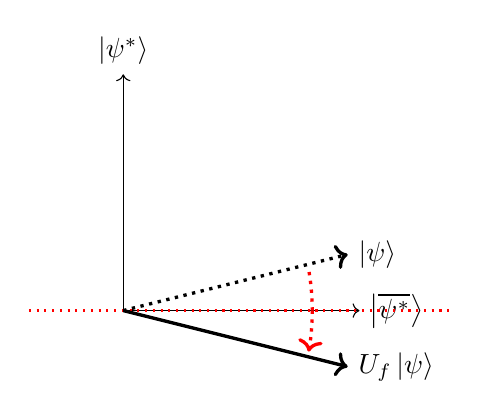
\begin{tikzpicture}[scale=0.6]
            \draw[->] (0,0) -- (5,0) node[anchor=west] {$\ket{\overline{\psi^*}}$};
            \draw[->] (0,0) -- (0,5) node[anchor=south] {$\ket{\psi^*}$};
    
            \draw[very thick, red, dotted]     (4,0) arc (0:10:5);
            \draw[very thick, red, dotted, ->] (4,0) arc (0:-10:5);
    
            \draw[thick, red, dotted] (-2, 0) -- (7,0);
    
    
            \draw[very thick, dotted, ->] (0,0) -- (4.75, 1.1875) node[anchor=west] {$\ket\psi$};
    
            \draw[very thick, ->] (0,0) -- (4.75, -1.1875) node[anchor=west] {$U_f\ket\psi$};
        \end{tikzpicture}
    }
    \subfigure[Diffusion]{
        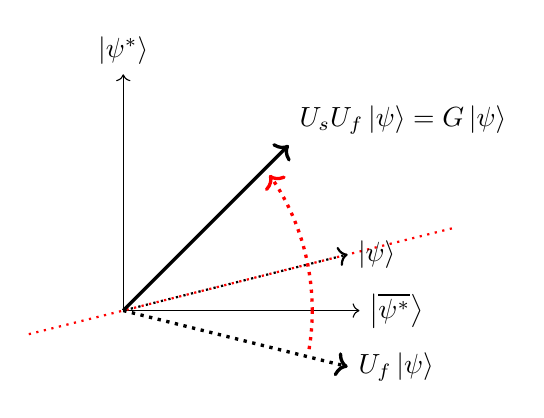
\begin{tikzpicture}[scale=0.6]
            \draw[->] (0,0) -- (5,0) node[anchor=west] {$\ket{\overline{\psi^*}}$};
            \draw[->] (0,0) -- (0,5) node[anchor=south] {$\ket{\psi^*}$};
    
            \draw[very thick, red, dotted, ->] (4,0) arc (0:35:5);
            \draw[very thick, red, dotted] (4,0) arc (0:-10:5);
    
            \draw[thick, red, dotted] (-2, -0.5) -- (7,1.75);
    
            \draw[thick, dotted, ->] (0,0) -- (4.75, 1.1875) node[anchor=west] {$\ket\psi$};
            \draw[very thick, dotted, ->] (0,0) -- (4.75, -1.1875) node[anchor=west] {$U_f\ket\psi$};
    
            \draw[very thick, ->] (0,0) -- (3.5, 3.5) node[anchor=south west] {$U_sU_f\ket\psi = G\ket\psi$};
        \end{tikzpicture}
    }
    \caption{All steps of Grover's algorithm visualized in the plane spanned by all valid configurations $\ket{\psi^*}$ and all non-valid configurations $\ket{\overline{\psi^*}}$}.
    \label{fig:bg:grover:steps}
\end{figure*}

\subsection{Quantum Computing}
\label{sec:bg:qc}
Quantum computing offers a new paradigm in computation, leveraging principles from quantum mechanics such as superposition and entanglement. 
Unlike classical computers, which rely on binary bits, quantum computers use qubits that can exist in multiple states simultaneously. 
While the technology is still in its early stages, it has the potential to provide advantages in specific problem areas like cryptography, optimization, and material science. 
However, it is important to note that quantum computers are not universally faster than classical computers and are best suited to particular types of computational problems.

The fundamental unit of quantum computing is the quantum gate, which is analogous to the classical logic gates utilized in traditional computing and serves as the basic component of a quantum circuit.
These gates facilitate the manipulation of qubits (quantum bits) through operations such as superposition and entanglement. 
It is noteworthy that certain quantum operations can negate one another, such that applying a gate followed by itself has no effect on the qubit's state. 
This property is pivotal for error correction and algorithm design.
Quantum circuits are composed of sequences of these gates, which permit the execution of complex computations through the parallel application of transformations on qubit states.

Two key metrics for assessing the complexity and efficiency of quantum circuits are depth and width.
\begin{description}
    \item[Width] The width of a quantum circuit is defined as the number of qubits utilized, and it determines the amount of information that the circuit can process in parallel.
    \item[Depth] The depth of a quantum circuit is a measure of the number of layers of gates applied sequentially.
    It is a reflection of the length of time required for the computation, as each layer can be executed simultaneously. 
\end{description}
A circuit with greater depth requires more time to execute, whereas a circuit with greater width can accommodate more complex states or parallel operations. 
The interplay between depth and width is crucial for understanding the resource requirements and potential limitations of quantum algorithms.

\subsection{Quantum Programming}
Qiskit is a widely used open-source quantum computing framework developed by IBM \cite{Qiskit}, designed to enable the creation, simulation, and execution of quantum circuits on both simulators and real quantum hardware. 
It provides a high-level Python interface for designing quantum algorithms, optimizing quantum circuits, and performing tasks such as quantum error correction, gate decomposition, and circuit transpilation. 
One of its core strengths is its ability to transpile circuits to match the constraints of actual quantum processors, such as gate set compatibility and qubit connectivity. 
This makes it highly versatile for both research and practical applications in quantum computing.

Complementing Qiskit is Quantum Assembly Language (QASM) \cite{cross2017openquantumassemblylanguage} \cite{OpenQASM3.0}, a low-level, hardware-agnostic language used to describe quantum circuits as a series of quantum gate operations and measurements.
QASM serves as the interface between high-level quantum algorithms and quantum hardware, translating the abstract structure of quantum circuits into executable instructions. 
This combination of Qiskit’s high-level capabilities and QASM’s precise control over quantum operations enables researchers and developers to experiment with quantum algorithms on various platforms, ranging from simulators to quantum hardware.

\subsection{Grover's Algorithm}
One of the most notable quantum algorithms is Grover's algorithm. 
Published by L. K. Grover in 1996 \cite{grover1996}, it exemplifies the power of quantum circuits by markedly accelerating the search process in unsorted databases, offering a quadratic speedup compared to classical algorithms. 
As searching solutions to logical formulae can be translated into finding possible solutions to the formula in a database containing all possible variable assignments, it can be seen that Grover's algorithm can also be used to solve logical formulae.
Grover can be mainly divided into three important steps

\begin{enumerate}
    \item \textbf{Preparation:} Prepares all $n$ non-ancilla qubits into a superposition state $\ket\psi$ consisting of $2^n$ possible states. In the context of Software Product Lines, $n$ describes the amount of features.
    \item \textbf{Oracle:} Marks all states that are valid solutions of our problem by negating their phase. In our context this means to mark all states that are valid configurations of our feature model. In a mathematical context this means to multiply our state $\ket\psi$ by the oracle operator/matrix $U_f$ resulting in our temporary state $U_f\ket\psi$.
    \item \textbf{Diffusion:} In the final step of Grover's algorithm we take the state $U_f\ket\psi$ and reflect it about the prepared state $\ket\psi$. Mathematically this means we multiply by another operation matrix $U_s$, giving us the state $U_sU_f\ket\psi$.
\end{enumerate}

This process is visualized in Figure \ref{fig:bg:grover:steps}. It displays the current state of our quantum system as a bold arrow in the plane of all possible $2^n$ configurations.
This plane is spanned by the two states $\ket{\psi^*}$ which describes a state consisting only of \textit{valid} configurations of our feature model, and state $\ket{\overline{\psi^*}}$ which consists of all \textit{invalid} configurations.
The last two steps, namely \textit{Oracle} ($U_f$) and \textit{Diffusion} ($U_s$) together are also called a \textit{Grover iteration} ($U_sU_f$).
This Grover iteration has to be repeated for  $\sim\frac{\pi}{4}\sqrt{N/M}$ solutions, where $N=2^n$ is the number of all \textit{possible} configurations, while $M$ describes all \textit{valid} configurations.



\begin{table}
    \centering
    \begin{tabular}{c|l|p{2.5cm}}
         Rule & Feature model primitive & propositional term\\
         \hline
         \hline
         1&$r$ is root feature & $r$\\
         \hline
         2&$f_1$ is \textit{mandatory} sub(-feature) of $f$ & $f_1 \Longleftrightarrow f$\\
         \hline
         3&$f_1$ is \textit{optional} sub of $f$ & $f_1 \Longrightarrow f$\\
         \hline
         4&$f_1,\dots,f_n$ \texttt{OR}-subs of $f$ & $f_1 \lor \dots \lor f_n \Longleftrightarrow f$\\
         \hline
         5&$f_1,\dots,f_n$ \texttt{XOR}-subs of $f$ & $f_1 \lor \dots \lor f_n \Longleftrightarrow f \newline \land \bigwedge\limits_{i<j}\lnot(f_i\land f_j)$\\
         \hline
         6&$f_1$ requires $f_2$ & $f_1 \Longrightarrow f_2$\\
         \hline
         7&$f_1$ excludes $f$ & $\lnot (f_1 \land f_2)$\\
    \end{tabular}
    \caption{Feature model primitives and their corresponding, propositional conjunction term.}
    \label{tab:bg:thesis:feature-table}
\end{table}
\section{State of the Art}
This subsection will provide the necessary background knowledge of our previous work \cite{thesis-marwin-kadner}, which this paper extends.
In reference to the cited thesis, we introduced a method for translating feature models that does not necessarily adhere to the CNF (Conjunctive Normal Form) format. Table \ref{tab:bg:thesis:feature-table} shows this translation.
Instead, it employs a propositional representation that encompasses a broader range of logical operators, not only including the classical \texttt{NOT}, \texttt{AND}, and \texttt{OR} gates but also proposing a quantum-equivalent interpretation for the gates \texttt{Implication}, \texttt{Equivalence} and \texttt{XOR}.

\begin{description}
    \item[Implication] The new implementation of an \texttt{Implication} gate is equal to an optimized version of the NNF version.
    A quantum circuit of this can be seen in Figure \ref{fig:bg:thesis:implication}. 

    \begin{figure}[H]
        \centering
        \subfigure[$\lnot f_1 \lor f$]{
        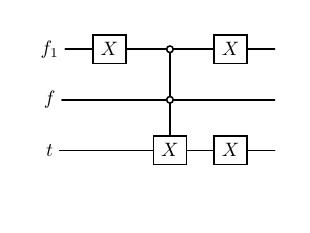
\begin{tikzpicture}
            \node[scale=0.7]{
                \begin{quantikz}
                    f_1~ & \gate{X} & \octrl{2} & \gate{X} & \\
                    f~ & & \octrl{0} & &\\
                    t~ & & \gate{X} & \gate{X} & \\ 
                \end{quantikz}
            };
        \end{tikzpicture}
        }
        \subfigure[$\lnot (f_1\land\lnot f)$]{
            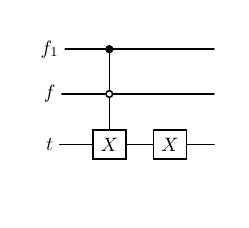
\begin{tikzpicture}
                \node[scale=0.7]{
                    \begin{quantikz}
                        f_1 ~ & \ctrl{2} &  & \\
                        f ~ & \octrl{0} &  & \\
                        t ~ & \gate{X} & \gate{X} & \\
                    \end{quantikz}
                };
            \end{tikzpicture}
        }
        \caption[Implication implementation]{
            Comparison of two alternative implementations of implication using quantum gates.}
        \label{fig:bg:thesis:implication}
    \end{figure} 

    \item[Equivalence]
    If we take a look at Table \ref{tab:bg:thesis:feature-table}, we can see that our \texttt{Equivalence} gate is either used to act on two input qubits, or a conjunction of input qubits and a single qubit.

    Our gate circuit for both of these cases can be seen in Figure \ref{fig:bg:thesis:equivalence-circuit}. 
    
    \begin{figure}[H]
        \centering
        \subfigure[$a \Leftrightarrow b$]{
            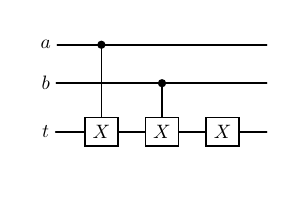
\begin{tikzpicture}
                \node[scale=0.7]{
                    \begin{quantikz}
                        a~ &\ctrl{2}&&& \\
                        b~ &&\ctrl{1}&& \\
                        t~ &\gate{X}&\gate{X}&\gate{X}& \\
                    \end{quantikz}
                };
            \end{tikzpicture}
        }
        \subfigure[$\bigvee\limits_{i=1\dots n}a_i \Leftrightarrow b$]{
            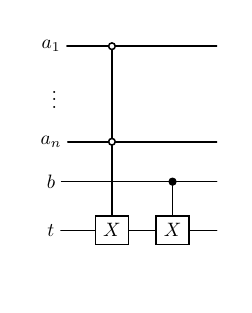
\begin{tikzpicture}
                \node[scale=0.7]{
                    \begin{quantikz}
                        a_1~ &\octrl{4}&&\\
                        \vdots \\
                        a_n~ &\octrl{2}&&\\
                        b~ &&\ctrl{1}& \\
                        t~ &\gate{X}&\gate{X}& \\
                    \end{quantikz}
                };
            \end{tikzpicture}
        }
        \caption[Equivalence Gate Circuit]{Example circuits for both rules that include an \texttt{Equivalence}.}.
        \label{fig:bg:thesis:equivalence-circuit}
    \end{figure}

    \item[XOR]
    While normally a $n$-ary \texttt{XOR} turns on for an uneven amount of toggled input bits, in the context of this paper a $n$-ary \texttt{XOR} refers to an operation that flips it’s target when only a single input qubit is 1. 
    This is due to semantics of alternative groups in feature models.
    XOR operations on only 2 operands (qubits) are basically the negated version of our Equivalence gate, checking exclusive disjunction for n. 
    Rule 5 in Table \ref{tab:bg:thesis:feature-table}, however, shows that we have to operate with multiple ($n$) input qubits.
    The new implementation of \texttt{XOR} is introduced as 
    \textbf{Disjunction of possibilities}: 
    
    This is designed by building one term for each possibility, so n in total. For the $i$-th term we check if only the $i$-th qubit is active while the others are inactive.
    Finally we build an OR with all our term ancillas as controls. 
    As a formula this would look like:

    \begin{align}
        \bigvee_{i=0}^n \bigl( f_i \land \bigwedge_{\substack{j\neq i \\ j=0}}^{n}\lnot f_j\bigr) &= \left( f_0 \land \lnot f_1 \land \dots \lnot \land f_n \right) \nonumber\\
        & \left( \lor\lnot f_0 \land f_1 \land \lnot f_2 \land \dots \land \lnot f_n \right) \nonumber\\
        &\vdots\nonumber\\
        &\left( \lor\lnot f_0 \land \dots \land \lnot f_{n-1} \land f_n \right)
    \end{align}

    While this works, utilizing the fact that always only one of these terms can be achieved, helps us to drastically reduce the width. Figure \ref{fig:bg:thesis:xor-disjunction-circuit} shows this optimized circuit.

    \begin{figure}[H]
        \centering
        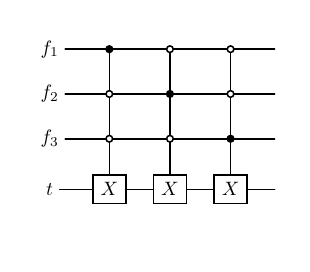
\begin{tikzpicture}
            \node[scale=0.7]{
                \begin{quantikz}
                    f_1~& \ctrl{3} & \octrl{3} & \octrl{3} & \\
                    f_2~& \octrl{0} & \ctrl{0} & \octrl{0} & \\
                    f_3~& \octrl{0} & \octrl{0} & \ctrl{0} & \\
                    t~  & \gate{X} & \gate{X} & \gate{X} & \\
                \end{quantikz}
            };
        \end{tikzpicture}
        \caption{Optimized circuit for possibility disjunction for $n=3$.}
        \label{fig:bg:thesis:xor-disjunction-circuit}
    \end{figure}
    
    
\end{description}

\section{Implementation}
This implementation section outlines the practical steps and theoretical enhancements made to improve upon the work of \textit{Kadner et al.} \cite{thesis-marwin-kadner}.
It details optimizations at the quantum circuit and gate level, focusing on reducing circuit depth and width for better efficiency. 
We also provide insights into how these improvements were translated into code, bridging the gap between theory and practical application. 
By explaining both the conceptual and technical aspects, this section highlights the key strategies used to enhance the performance of Grover’s algorithm in the context of software product lines.
% \subsection{Refactoring}
% In the course of refactoring the existing implementation proposed by \textit{Kadner et al.} and \textit{Ammermann et al}.\cite{ammermann2023quantumcomputingimproveuniform, thesis-marwin-kadner}, several established principles were applied to improve the codebase’s structure, readability, and maintainability. 
% The Single Responsibility Principle was adopted to ensure that each function and class is designed with a specific, well-defined responsibility, thereby enhancing modularity and easing the debugging process. 
% To address code duplication, the DRY (Don't Repeat Yourself) principle was implemented by consolidating repetitive logic into reusable functions and classes, thereby reducing redundancy. 
% Additionally, code readability was enhanced through the use of descriptive variable and function names, consistent indentation, and the inclusion of comments to elucidate complex logic. 
% Furthermore, refactoring patterns such as method and class extraction were employed to decompose large, monolithic functions and classes into more manageable components. 
% These refinements not only contributed to a cleaner and more organized codebase but also facilitated improved testing and future modifications.
\subsection{Redundant Operations}

\newcommand{\bm}[4]{\begin{bmatrix}#1&#2\\#3&#4\end{bmatrix}}
\newcommand{\Xgate}{\bm{0}{1}{1}{0}}
\newcommand{\Hgate}{-\frac{1}{\sqrt{2}}\bm{1}{1}{1}{-1}}

In Quantum Computing, some operations are self-inverse, meaning that their operation matrix is involutory. For example, given the Hadamard Gate $H =\Hgate$ we see that multiplying H by itself will result in an identity matrix:
\begin{align}
    H^2 &= \Hgate \Hgate \nonumber\\
    &= \frac{1}{2}\bm{2}{0}{0}{2} = \bm{1}{0}{0}{1}\
\end{align}
To further optimize the quantum circuit, we eliminate these self-inverse operations. 
This is done by creating a two-dimensional array that tracks the operations for each qubit. 
We then iteratively traverse the array, identifying and removing successive pairs of self-inverting gates. 
This process is repeated until no more such pairs are found. 
While this optimization reduces the circuit depth in the generated QASM output, it does not affect the depth when transpiled using Qiskit, since its \textit{transpile()} method inherently removes redundant gates. 
Nevertheless, this improvement results in a shorter depth in the QASM representation, potentially providing future flexibility by reducing dependencies on specific frameworks or libraries.

\subsection{Lookup Tables}
\label{sec:impl:lookup-tables}
It is not uncommon for multiple constraints within one feature model to exhibit similarities in their constituent parts, given that features often interact in ways that are not mutually exclusive.
For example, certain features may be required or excluded together across different constraints, leading to the emergence of repeated patterns in the Boolean formulae.
These repeated patterns are also represent in the previous implementation of the quantum circuit.
As shown in \autoref{tab:bg:thesis:feature-table} all constraints require one or even multiple additional qubits, so called \textit{ancilla qubits}. 
These qubits store temporary results that are needed for entangling the constraint to the final result state.
The repeated patterns thus cause some ancilla qubits to store the same state and hence be duplicates.

This is where our optimization comes in. When creating the circuit, we try to build a lookup table for all previously created (ancilla) qubits and what logical formulae they represent. 
When creating the qubits for constraints we look for qubits that store the same state as is required for our constraint.
If such qubit is found, we use it instead of creating a new one, saving on both depth and width.
When looking at our example \textit{Sandwich} feature model shown in Figure \ref{fig:bg:spl:sandwich-imply-model}, we can see that both constraints contain the term "Gouda $\land$ Salami".

Figure \ref{fig:impl:lookup-table-comparison} shows the comparison of the resulting quantum circuits that represent these constraints.
Subfigure (a) was generated using the previous version of the implementation, whereas (b) was created using a revised version that incorporates lookup tables.
We can see that the circuit width of our new implementation was reduced by one qubit.
This was due to the removal of the duplicate qubit "Gouda $\land$ Salami" in the old implementation.
In the new implementation both final constraints qubits ("Toast $\implies$ (Gouda $\land$ Salami)" and "Full Grain $\implies$ (Gouda $\land$ Salami)") use the same qubit as control instead of creating a new one as it was done in the old implementation. 

\begin{figure}
    \subfigure[Old Implementation]{
    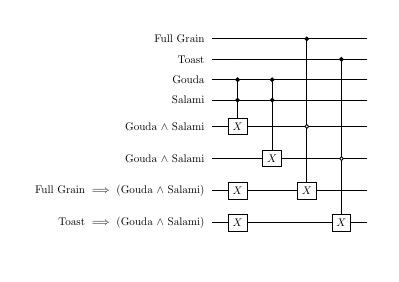
\begin{tikzpicture}
        \node[scale=0.4]{
            \begin{quantikz}[scale=0.5]
                \lstick{Full Grain}~ & && \ctrl{6}&&\\
                \lstick{Toast}~ & &&&\ctrl{6}&\\
                \lstick{Gouda}~ & \ctrl{2} & \ctrl{3} &&&\\
                \lstick{Salami}~ & \ctrl{0} & \ctrl{0} &&&\\
                \lstick{Gouda $\land$ Salami}~ & \gate{X} &&\octrl{0}&&\\
                \lstick{Gouda $\land$ Salami}~ & & \gate{X}&&\octrl{0}&\\
                \lstick{Full Grain $\implies$ (Gouda $\land$ Salami)}~ &\gate{X}&&\gate{X}&&\\
                \lstick{Toast $\implies$ (Gouda $\land$ Salami)}~ &\gate{X}&&&\gate{X}&\\
            \end{quantikz}
        };
    \end{tikzpicture}
    }
    \subfigure[New Implementation]{
    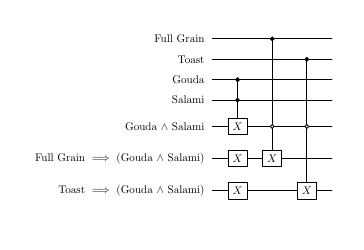
\begin{tikzpicture}
        \node[scale=0.4]{
            \begin{quantikz}
                \lstick{Full Grain}~ && \ctrl{5}&&\\
                \lstick{Toast}~ &&&\ctrl{5}&\\
                \lstick{Gouda}~ & \ctrl{2} &&&\\
                \lstick{Salami}~ & \ctrl{0} &&&\\
                \lstick{Gouda $\land$ Salami}~ & \gate{X} &\octrl{0}&\octrl{0}&\\
                \lstick{Full Grain $\implies$ (Gouda $\land$ Salami)}~ &\gate{X}&\gate{X}&&\\
                \lstick{Toast $\implies$ (Gouda $\land$ Salami)}~ &\gate{X}&&\gate{X}&\\
            \end{quantikz}
        };
    \end{tikzpicture}
    }
    \caption{Quantum circuits satisfying the constraints of our example feature model \ref{fig:bg:spl:sandwich-imply-model}.}
    \label{fig:impl:lookup-table-comparison}
\end{figure}

% \subsection{Improving Grover's Iteration (Optional)}
% Due to time limitations, the optional task of improving and optimizing Grover's algorithm could not be completed in this paper. 
% Instead, we reference the approach proposed by \textit{Xiang Li et al. (2023)}, who  published \cite{li2023resource} in which they discuss possible methods for increasing efficiency of Grover's algorithm.
% They proposed three different methods, one they call \textit{W-cycle Oracle}.
% It allows the creation of at most $2^m$ boolean equations using only $m$ ancilla qubits, at the cost of a deeper circuit.
% Another one is \textit{Oracle compression} that compresses circuits by removing redundant gates that cancel each other out.
% And the last method for which they apply a different Oracle in each iteration based on a subset of all solutions to reduce the depth, is called \textit{Randomized Grover's Algorithm}.
% The idea for this method is that in each iteration the amplitudes for valid solutions will always get amplified and the solutions to the specific subset of problems will get amplified but will get reduced again in other iterations.
% However, they concluded that convergence is not always guaranteed.
% As our thesis focuses more on the reduction of length of the Boolean formula theirs focuses on the technical implementation of the Grover oracle and can thus be seen as an additional optimization on top of our thesis.



\section{Related Work}
In the following section we will take a look into current literature on this topic.
This is important as it positions our thesis within the larger quantum computing landscape and shows how it differs from other work on the topic.



\textit{Hangleiter and Eisert} explore various random sampling techniques in quantum circuits and their computational advantages in their paper \cite{Hangleiter_2023}. 
They define quantum random sampling as the process of obtaining samples from random quantum computations. 
However, this paper takes a different approach. 
Instead of focusing on random quantum computations, it addresses the challenge of generating uniform random samples from a distribution under specific constraints, a task that cannot be accomplished solely through random quantum computation.

In the context of Grover's algorithm, recent advancements have explored ways to enhance its efficiency. \textit{Xiang Li et al. (2023)} proposed in \cite{li2023resource} several optimization techniques, including the W-cycle Oracle, Oracle compression, and Randomized Grover's Algorithm to reduce circuit complexity and increase computational efficiency.
\begin{description}
    \item[W-cycle Oracle]
    It allows the creation of at most $2^m$ boolean equations using only m ancilla qubits, at the cost of a deeper circuit.
    \item[Oracle Compression]
    Oracle Compression is the same type of optimization as we are proposing in this paper by removing redundant gates.
    \item[Randomized Grover's Algorithm]
    The idea for this method, is that in each iteration the amplitudes for valid solutions will always get amplified and the solutions to the specific subset of problems will get amplified but will get reduced again in other iterations.
    However, they concluded that convergence is not always guaranteed.
\end{description}
These approaches focus on improving the implementation of the Grover oracle by reducing the number of ancilla qubits, eliminating redundant gates, and applying a randomized oracle to amplify solutions in different iterations, albeit without guaranteed convergence. 
While these optimizations fall beyond the scope of this paper, which centers on reducing the depth and width of a giving implementation, they represent promising complementary strategies for further improving Grover's algorithm.

\begin{table*}
    \centering
    \begin{tabular}{c|c||c|c||c|c}
        Feature Model & \# of features & Previous Depth & New Depth & Previous Width & New Width\\
        \hline \hline
        Car & 10 & 32 & 32 & 21 & 21 \\
        Sandwich & 11 & 32 & 30 & 35 & 35\\
        Bike & 54 & 58 & 58 & 92 & 92\\
        axTLS & 96 & 304 & 304 & 296 & 271\\
        cLib & 313 & 902 & 856 & 1103 & 909\\
        BusyBox & 854 & 2998 & 2794 & 2558 & 2390 \\
        Toolkit & 1179 & 27956 & 4736 & 22449 & 2558
    \end{tabular}
    \caption{Width and Depth of our test models and their respective size in amount of features (\# of features). The depth was calculated by transpiling the circuit onto the statevector backend. We compare the old implementation presented in \cite{thesis-marwin-kadner} and the new implementation introduced in this paper.}
    \label{tab:eval:depth-width}
\end{table*}

\section{Evaluation}
In this chapter, we evaluate our implementation and compare it to the previous implementation by \textit{Kadner et al.} in \cite{thesis-marwin-kadner}.
We evaluate based on two critical quantum circuit metrics: Depth and Width.
These metrics, which are crucial for understanding the efficiency and scalability of quantum circuits, are discussed in detail in Section 2.2 of our Background.
Finally, we compare the results with our previous work \cite{thesis-marwin-kadner} and assess on possible improvements or deteriorations.

\subsection{Methodology}
The methodolgy follows the approach outlined by \textit{Ammermann et al.} in \cite{ammermann2023quantumcomputingimproveuniform} and \textit{Kadner et al.} in \cite{thesis-marwin-kadner}.
For proper benchmarking and comparison we use the same feature models as in the previous work.
These are feature models by the BURST benchmarking suite \cite{burst-suite} and examples by the software product line tool FeatureIDE \cite{feature_ide}.
We begin by creating a QASM output for both the previous implementation and our proposed implementation.
Afterwards we parse this output into a Qiskit object using the \textit{parse()} method provided by Qiskit in their Python module \texttt{qiskit\_qasm3\_import}.
Finally working on a Qiskit object allows us to utilize the \textit{depth()} and \textit{width()} methods it provides.
The evaluation will focus on comparing the performance of our implementation against previous work, highlighting improvements in both circuit depth and width.


\subsection{Depth}
To evaluate the depth of our new implementation, we performed a comparison between the computed depth of our approach and the one presented in the reference work \cite{thesis-marwin-kadner, ammermann2023quantumcomputingimproveuniform}. 
The results, as shown in Table \ref{tab:eval:depth-width}, indicate a significant improvement in depth, especially in the case of larger feature models. 
These larger models tend to introduce more complex constraints and, as a result, often contain more duplicated qubits in the previous implementation. 
The increased number of duplicated qubits provides an opportunity for our new method to apply more efficient optimization techniques, leading to a more substantial reduction in circuit depth.
In contrast, smaller feature models with fewer constraints and duplicated qubits do not offer the same level of optimization potential, resulting in relatively smaller improvements. 
This demonstrates that the benefits of our implementation become more pronounced as the complexity of the feature models increases, highlighting its effectiveness for scaling to more complex quantum circuits.



\subsection{Width}
We observe similar improvements in the width of our new implementation as in the circuit depth. As discussed in Section \ref{sec:impl:lookup-tables}, our approach significantly reduces the need to duplicate qubits, resulting in significant width savings. By minimizing qubit duplication, our method optimizes resource utilization, especially in more complex circuits. Table \ref{tab:eval:depth-width} illustrates that these gains are most evident in larger feature models, which are more prone to duplicated logical terms. In such models, the elimination of redundant qubits has a greater impact, resulting in a significant reduction in circuit width. Conversely, smaller feature models, which typically have fewer duplications, show less dramatic improvements. Nevertheless, the results show that our implementation is particularly beneficial for feature models of high complexity, where it effectively reduces both the number of qubits and the circuit overhead.


\section{Conclusion}
In conclusion, this paper has presented significant improvements to the application of Grover's algorithm for uniform random sampling, particularly in the context of software product lines (SPLs).
By optimizing quantum circuits through the removal of redundant operations, the reuse of qubits, and the development of more efficient logic gate structures, the proposed approach reduces both the depth and width of quantum circuits. 
These optimizations enhance the resource efficiency of the algorithm and demonstrate scalability across larger feature models, as evidenced by the evaluation. 
Ultimately, these advancements facilitate the practical application of quantum computing for solving complex problems in software engineering, paving the way for future innovations in SPL management and testing.
%%
%% The acknowledgments section is defined using the "acks" environment
%% (and NOT an unnumbered section). This ensures the proper
%% identification of the section in the article metadata, and the
%% consistent spelling of the heading.
\begin{acks}
To Robert, for the bagels and explaining CMYK and color spaces.
\end{acks}

%%
%% The next two lines define the bibliography style to be used, and
%% the bibliography file.
\bibliographystyle{ACM-Reference-Format}
\newpage
\bibliography{sample-base}


%%
%% If your work has an appendix, this is the place to put it.

\end{document}
\endinput
%%
%% End of file `sample-sigconf.tex'.
